\documentclass[11pt, a4paper]{article}

% --- Packages ---
\usepackage[utf8]{inputenc}
\usepackage[T1]{fontenc}
\usepackage{mathptmx} % Times New Roman font for professional document typography
\usepackage{graphicx}
\usepackage[margin=0.8in]{geometry}
\usepackage{xcolor}
\usepackage{titlesec}
\usepackage{enumitem}
\usepackage{float}
\usepackage{booktabs}
\usepackage{multirow}
\usepackage{array}
\usepackage{url}
\usepackage[colorlinks=true, linkcolor=amritaMaroon, urlcolor=amritaMaroon, citecolor=amritaMaroon]{hyperref}
\usepackage{tikz}
\usetikzlibrary{calc,arrows.meta,positioning,shapes.geometric}

\graphicspath{{../}{./}}

% --- Amrita Colors ---
\definecolor{amritaMaroon}{HTML}{A4123F}
\definecolor{boxBg}{HTML}{F8F9FA}
\definecolor{borderGray}{HTML}{D1D5DB}
\definecolor{nodeBlue}{HTML}{E8F0FE}
\definecolor{accentGreen}{HTML}{0D9488}

% --- Title & Section Formatting ---
\titlespacing*{\section}{0pt}{12pt}{4pt}
\titlespacing*{\subsection}{0pt}{8pt}{3pt}
\titleformat{\section}{\large\bfseries\color{amritaMaroon}}{\thesection}{0.8em}{}
\titleformat{\subsection}{\normalsize\bfseries\color{amritaMaroon}}{\thesubsection}{0.6em}{}

\pagestyle{plain}

\begin{document}

% ==========================================
% HEADER & TITLE BLOCK
% ==========================================
\noindent
\begin{minipage}{\textwidth}
    \centering
    {\Large \textbf{\textcolor{amritaMaroon}{
    AMRITA VISHWA VIDYAPEETHAM \\
    SCHOOL OF COMPUTING \\
    DEPARTMENT OF COMPUTER SCIENCE AND ENGINEERING \\
    }}}
    \vspace{0.2cm}
    {\large \textbf{M.A.C.H. AI: MULTIMODAL ACADEMIC COGNITIVE HUB}} \\[0.08cm]
    {\normalsize \textbf{A Fine-Tuned Graph-RAG Framework for Campus Knowledge Systems}} \\[0.12cm]
    \textbf{23CSE498 -- Project Phase II (External Review)} \quad | \quad \textbf{Team Number: G081} \\
    \today
\end{minipage}

\vspace{0.3cm}
\hrule
\vspace{0.3cm}

% --- Team & Guide Details ---
\noindent
\begin{center}
    \renewcommand{\arraystretch}{1.40}
    \setlength{\tabcolsep}{6pt}
    \begin{tabular}{|l|p{4.8cm}|p{4.6cm}|p{3.2cm}|}
        \hline
        \multicolumn{2}{|c|}{\textbf{Team Members}} & \textbf{Project Guide} & \textbf{Project Type} \\
        \hline
        \small CB.SC.U4CSE23505 & \small \raggedright A. Chandra Vamsi &
        \multirow{4}{=}{\raggedright \small \textbf{Dr. Shanmuga Priya S} \newline \textit{Assistant Professor (Sl.Gd.), \newline Dept. of CSE}} &
        \multirow{4}{=}{\raggedright \small \textbf{Type 3} \newline Software-Based Project} \\ \cline{1-2}
        \small CB.SC.U4CSE23508 & \small B. Prem Sai Charan & & \\ \cline{1-2}
        \small CB.SC.U4CSE23530 & \small M. Pavan Prem Prabhas & & \\ \cline{1-2}
        \small CB.SC.U4CSE23568 & \small P. Tirupati Reddy & & \\
        \hline
    \end{tabular}
\end{center}
\vspace{0.2cm}

\section{Abstract}
\noindent
Academic institutions produce substantial volumes of heterogeneous, unstructured, and semi-structured documents, including course curriculum handbooks, academic calendars, examination seating charts, timetable schedules, and past year question papers (PYQs). Conventional document search solutions and third-party commercial cloud Large Language Models (LLMs) suffer from domain hallucinations, lose hierarchical course prerequisite dependencies, and risk student data privacy. This project introduces \textbf{M.A.C.H. AI (Multimodal Academic Cognitive Hub)}, a full-stack, 100\% air-gapped on-premise software platform powered by a hybrid Graph Retrieval-Augmented Generation (Graph-RAG) architecture. The system features a decoupled 4-tier design: a responsive presentation tier (Vanilla HTML5/ES6, KaTeX, Web Speech API, and PWA service worker), an asynchronous FastAPI service layer with JWT role-based access control, and a hybrid persistence tier combining PostgreSQL 16 with pgvector (\texttt{halfvec} 768-dimension HNSW indexing) and Neo4j 5.24 Community Graph Database. The platform employs a deterministic dual-layer intent router that executes curriculum and prerequisite lookups directly in Neo4j without invoking an LLM ($<50$\,ms latency), while routing complex inquiries through a Reciprocal Rank Fusion (RRF) pipeline that combines dense vector similarity with sparse GIN tsvector matching. Generative responses are streamed via Server-Sent Events (SSE) from a quantized local multimodal model (\texttt{gemma4:12b-it-qat}) running on Ollama. The complete software system was validated through an automated test suite of 110 test cases across unit, integration, system, and security levels (100\% pass rate in 4.14\,s), confirming full architectural stability and production readiness.

% =========================================================================
% SECTION 2: PROBLEM DEFINITION, MOTIVATION & SRS (5 MARKS)
% =========================================================================
\section{Problem Definition, Motivation \& Software Requirements Specification (SRS)}

\subsection{Problem Definition \& Institutional Motivation}
\noindent
In modern academic environments, students and faculty frequently navigate disparate document repositories to locate course prerequisites, syllabus modules, examination seating schedules, and past question papers. Traditional vector-based Retrieval-Augmented Generation (RAG) approaches \cite{gao2023rag,izacard2021leveraging} fail in two fundamental aspects: (1) chunk-based vector search breaks hierarchical relationships (Course $\rightarrow$ Unit $\rightarrow$ Topic $\rightarrow$ Prerequisite) \cite{sitaram2022curriculum,edge2024graphrag}, leading to factual errors; and (2) reliance on external cloud APIs compromises institutional data privacy. Furthermore, questions in engineering question papers often depend heavily on visual circuit schematics and mathematical formulas, which cannot be represented effectively by text-only parsers. M.A.C.H. AI resolves these challenges through a localized Graph-RAG system that guarantees deterministic accuracy on curriculum data, zero external data leakage, and automated visual diagram extraction.

\subsection{Product Scope, Actors \& Core Use Cases}
\begin{itemize}[noitemsep, topsep=2pt]
    \item \textbf{Software Scope:} Privacy-preserving, on-premise academic assistant for university curriculum handbooks, administrative circulars, timetables, seating arrangements, and past question papers.
    \item \textbf{User Roles / Actors:}
    \begin{enumerate}[noitemsep]
        \item \textit{Student:} Interacts with the interface to query syllabus details, prerequisites, topic-specific exam questions filtered by Bloom's Taxonomy levels, and exam hall seating.
        \item \textit{Academic Administrator:} Ingests institutional circulars, synchronizes graph entities, and monitors automated retrieval evaluation scorecards.
    \end{enumerate}
    \item \textbf{Core Use Cases:}
    \begin{enumerate}[noitemsep, topsep=2pt]
        \item \textit{UC-01 (Deterministic Syllabus \& Prerequisite Query):} Student queries course prerequisites or syllabus units. The system resolves the course code, queries Neo4j directly, and returns structured units in $<50$\,ms without consuming GPU tokens.
        \item \textit{UC-02 (Topic-Specific PYQ Retrieval with Visual Diagram Cropping):} Student asks for questions on a specific concept (e.g., \textit{"Mesh Analysis"}). The system executes contrastive topic filtering to suppress unrelated circuit problems, retrieves exact questions from PostgreSQL, and serves high-resolution auto-cropped circuit schematics alongside KaTeX-rendered equations.
        \item \textit{UC-03 (Administrative Document QA):} Actor queries exam seating or calendar dates. The system extracts structured tabular metadata and returns exact schedule details.
    \end{enumerate}
\end{itemize}

\subsection{Functional \& Non-Functional Requirements}
\begin{table}[H]
    \centering
    \footnotesize
    \renewcommand{\arraystretch}{1.25}
    \begin{tabular}{|c|p{3.0cm}|p{9.4cm}|}
        \hline
        \textbf{Req. ID} & \textbf{Category} & \textbf{Requirement Specification} \\
        \hline
        FR-01 & Curriculum Graph Traversal & The system shall deterministically extract course syllabus units, course outcomes (COs), and prerequisite paths from Neo4j without relying on LLM generation. \\
        \hline
        FR-02 & Hybrid Multimodal PYQ Search & The system shall retrieve past examination questions using Reciprocal Rank Fusion (RRF) across dense vector embeddings (\texttt{halfvec(768)}) and sparse BM25 keyword indices. \\
        \hline
        FR-03 & Automated Visual Cropping & The system shall identify bounding boxes of circuit diagrams and equations from question PDFs and serve high-resolution cropped PNG images to the user interface. \\
        \hline
        FR-04 & Contrastive Subtopic Filtering & The system shall distinguish between closely related concepts (e.g., \textit{"combination of capacitors"} vs. \textit{"combination of resistors"}) and penalize cross-topic contamination. \\
        \hline
        FR-05 & Admin Ingestion \& Evaluation & The system shall support multipart document ingestion and provide automated evaluation metrics using the RAGAS framework \cite{es2024ragas}. \\
        \hline
        NFR-01 & Response Latency & Deterministic graph lookups shall execute in $<50$\,ms; first token delivery (TTFT) for generative queries shall be under $450$\,ms via Server-Sent Events (SSE). \\
        \hline
        NFR-02 & Data Privacy \& Security & 100\% on-premise execution with no external API calls; passwords hashed using Bcrypt; API endpoints guarded by JWT authentication and IP rate limiting. \\
        \hline
        NFR-03 & Memory Efficiency & The vector persistence layer shall utilize 16-bit half-precision floats (\texttt{halfvec}), reducing database RAM and storage footprint by 50\% relative to standard \texttt{vector(768)}. \\
        \hline
    \end{tabular}
    \caption{Software Functional and Non-Functional Requirements Specification}
\end{table}

% =========================================================================
% SECTION 3: SOFTWARE ARCHITECTURE & SYSTEM DESIGN
% =========================================================================
\section{Software Architecture \& System Design}

\subsection{High-Level System Architecture}
\noindent
The software adopts a decoupled, multi-tier service-oriented architecture designed for maximum modularity, low latency, and ease of maintainability. Figure~1 illustrates the flow from the client tier through the API gateway, core orchestration engine, and persistent storage layers.

\begin{figure}[H]
    \centering
    \resizebox{0.96\linewidth}{!}{
        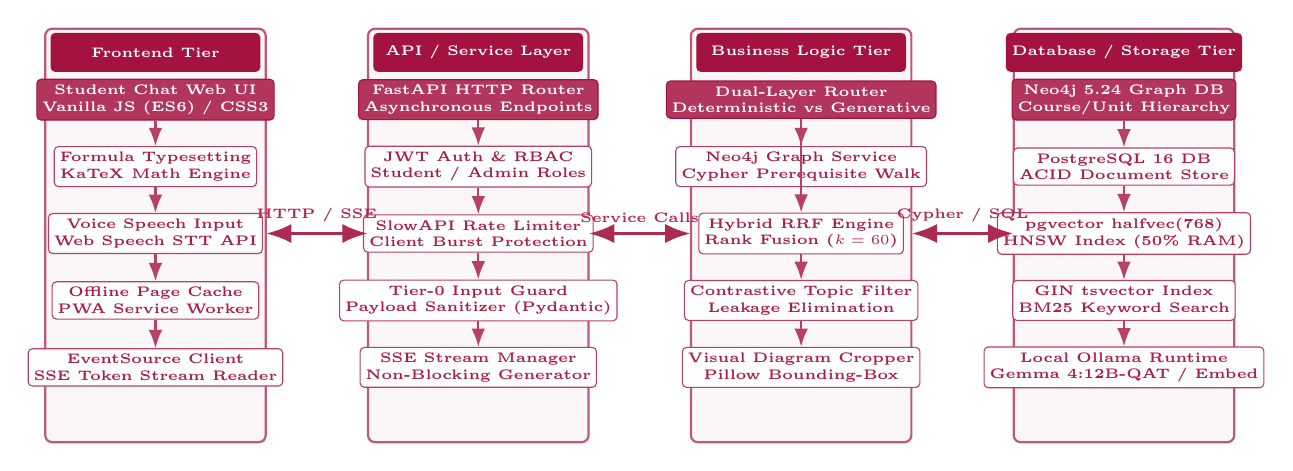
\begin{tikzpicture}[
            font=\tiny,
            tierbox/.style={draw=amritaMaroon!70, fill=amritaMaroon!4, rounded corners=2.5pt, thick},
            tierhdr/.style={draw=amritaMaroon, fill=amritaMaroon, text=white, rounded corners=1.5pt,
                            minimum width=2.65cm, minimum height=0.48cm, align=center, font=\tiny\bfseries, inner sep=2pt},
            subnode/.style={draw=amritaMaroon!80, fill=white, text=amritaMaroon!95, rounded corners=1.5pt,
                            minimum width=2.5cm, minimum height=0.44cm, align=center, font=\tiny\bfseries, inner sep=2pt},
            subnodeDark/.style={draw=amritaMaroon, fill=amritaMaroon!85, text=white, rounded corners=1.5pt,
                                minimum width=2.5cm, minimum height=0.44cm, align=center, font=\tiny\bfseries, inner sep=2pt},
            arr/.style={->, >=Latex, thick, color=amritaMaroon!80},
            tierArr/.style={<->, >=Latex, line width=1.4pt, color=amritaMaroon!90}
        ]

            %% ==========================================
            %% 1. FRONTEND TIER
            %% ==========================================
            \draw[tierbox] (-1.4, -4.1) rectangle (1.4, 1.15);
            \node[tierhdr] at (0, 0.85) {Frontend Tier};
            \node[subnodeDark] (fe1) at (0,  0.25) {Student Chat Web UI\\Vanilla JS (ES6) / CSS3};
            \node[subnode]     (fe2) at (0, -0.60) {Formula Typesetting\\KaTeX Math Engine};
            \node[subnode]     (fe3) at (0, -1.45) {Voice Speech Input\\Web Speech STT API};
            \node[subnode]     (fe4) at (0, -2.30) {Offline Page Cache\\PWA Service Worker};
            \node[subnode]     (fe5) at (0, -3.15) {EventSource Client\\SSE Token Stream Reader};
            \draw[arr](fe1)--(fe2); \draw[arr](fe2)--(fe3);
            \draw[arr](fe3)--(fe4); \draw[arr](fe4)--(fe5);

            %% ==========================================
            %% 2. API / SERVICE LAYER
            %% ==========================================
            \draw[tierbox] (2.7, -4.1) rectangle (5.5, 1.15);
            \node[tierhdr] at (4.1, 0.85) {API / Service Layer};
            \node[subnodeDark] (ap1) at (4.1,  0.25) {FastAPI HTTP Router\\Asynchronous Endpoints};
            \node[subnode]     (ap2) at (4.1, -0.60) {JWT Auth \& RBAC\\Student / Admin Roles};
            \node[subnode]     (ap3) at (4.1, -1.45) {SlowAPI Rate Limiter\\Client Burst Protection};
            \node[subnode]     (ap4) at (4.1, -2.30) {Tier-0 Input Guard\\Payload Sanitizer (Pydantic)};
            \node[subnode]     (ap5) at (4.1, -3.15) {SSE Stream Manager\\Non-Blocking Generator};
            \draw[arr](ap1)--(ap2); \draw[arr](ap2)--(ap3);
            \draw[arr](ap3)--(ap4); \draw[arr](ap4)--(ap5);

            %% ==========================================
            %% 3. BUSINESS LOGIC TIER
            %% ==========================================
            \draw[tierbox] (6.8, -4.1) rectangle (9.6, 1.15);
            \node[tierhdr] at (8.2, 0.85) {Business Logic Tier};
            \node[subnodeDark] (bl1) at (8.2,  0.25) {Dual-Layer Router\\Deterministic vs Generative};
            \node[subnode]     (bl2) at (8.2, -0.60) {Neo4j Graph Service\\Cypher Prerequisite Walk};
            \node[subnode]     (bl3) at (8.2, -1.45) {Hybrid RRF Engine\\Rank Fusion ($k=60$)};
            \node[subnode]     (bl4) at (8.2, -2.30) {Contrastive Topic Filter\\Leakage Elimination};
            \node[subnode]     (bl5) at (8.2, -3.15) {Visual Diagram Cropper\\Pillow Bounding-Box};
            \draw[arr](bl1)--(bl2); \draw[arr](bl1)--(bl3);
            \draw[arr](bl3)--(bl4); \draw[arr](bl4)--(bl5);

            %% ==========================================
            %% 4. DATABASE / STORAGE TIER
            %% ==========================================
            \draw[tierbox] (10.9, -4.1) rectangle (13.7, 1.15);
            \node[tierhdr] at (12.3, 0.85) {Database / Storage Tier};
            \node[subnodeDark] (db1) at (12.3,  0.25) {Neo4j 5.24 Graph DB\\Course/Unit Hierarchy};
            \node[subnode]     (db2) at (12.3, -0.60) {PostgreSQL 16 DB\\ACID Document Store};
            \node[subnode]     (db3) at (12.3, -1.45) {pgvector halfvec(768)\\HNSW Index (50\% RAM)};
            \node[subnode]     (db4) at (12.3, -2.30) {GIN tsvector Index\\BM25 Keyword Search};
            \node[subnode]     (db5) at (12.3, -3.15) {Local Ollama Runtime\\Gemma 4:12B-QAT / Embed};
            \draw[arr](db1)--(db2); \draw[arr](db2)--(db3);
            \draw[arr](db3)--(db4); \draw[arr](db4)--(db5);

            %% ==========================================
            %% INTER-TIER CONNECTIONS (<->)
            %% ==========================================
            \draw[tierArr] (1.4, -1.45) -- node[above, font=\tiny\bfseries, text=amritaMaroon!90] {HTTP / SSE} (2.7, -1.45);
            \draw[tierArr] (5.5, -1.45) -- node[above, font=\tiny\bfseries, text=amritaMaroon!90] {Service Calls} (6.8, -1.45);
            \draw[tierArr] (9.6, -1.45) -- node[above, font=\tiny\bfseries, text=amritaMaroon!90] {Cypher / SQL} (10.9, -1.45);

        \end{tikzpicture}
    }
    \caption{Full-Width Software System Architecture (Frontend $\longleftrightarrow$ API Layer $\longleftrightarrow$ Business Logic $\longleftrightarrow$ Database Tier)}
\end{figure}

\subsection{Database Schema \& Data Modeling}
\noindent
The persistence layer combines relational/vector storage in PostgreSQL 16 with a property graph in Neo4j 5.24 Community Edition, as modeled in Figure~2.

\begin{figure}[H]
    \centering
    \resizebox{0.95\linewidth}{!}{
        \begin{tikzpicture}[
            font=\tiny,
            table/.style={rectangle, draw=amritaMaroon, fill=white, rounded corners=1.5pt, thick, align=left, inner sep=4pt, text width=4.0cm},
            gnode/.style={rectangle, draw=accentGreen, fill=accentGreen!10, rounded corners=1.5pt, thick, align=left, inner sep=4pt, text width=4.0cm},
            arr/.style={->, >=Latex, thick, color=amritaMaroon!80}
        ]
            % Relational Tables
            \node[table] (users) at (0, 0) {
                \textbf{\textcolor{amritaMaroon}{users (PostgreSQL)}} \\
                \hline
                \underline{id}: UUID [PK] \\
                username: VARCHAR(50) [UNIQUE] \\
                password\_hash: VARCHAR(255) \\
                role: VARCHAR(20) [admin/student] \\
                created\_at: TIMESTAMP
            };

            \node[table] (pyq) at (0, -2.5) {
                \textbf{\textcolor{amritaMaroon}{pyq\_questions (PostgreSQL)}} \\
                \hline
                \underline{id}: INTEGER [PK] \\
                course\_code: VARCHAR(10) [INDEX] \\
                question\_text: TEXT \\
                marks: INTEGER \\
                bloom\_level: VARCHAR(10) \\
                tsv: TSVECTOR [GIN INDEX] \\
                embedding: HALFVEC(768) [HNSW]
            };

            % Neo4j Graph Nodes
            \node[gnode] (course) at (5.5, 0) {
                \textbf{\textcolor{accentGreen}{Course (Neo4j Node)}} \\
                \hline
                code: STRING [UNIQUE PK] \\
                name: STRING \\
                credits: INTEGER \\
                semester: INTEGER
            };

            \node[gnode] (unit) at (10.5, 0) {
                \textbf{\textcolor{accentGreen}{Unit (Neo4j Node)}} \\
                \hline
                unit\_number: INTEGER \\
                title: STRING
            };

            \node[gnode] (topic) at (10.5, -2.5) {
                \textbf{\textcolor{accentGreen}{Topic / SubTopic (Neo4j)}} \\
                \hline
                name: STRING \\
                keywords: LIST<STRING>
            };

            % Graph Relationships
            \draw[arr] (course) -- node[above, font=\tiny] {[:HAS\_UNIT]} (unit);
            \draw[arr] (unit) -- node[right, font=\tiny] {[:COVERS]} (topic);
            \draw[arr] (course) to [out=140,in=40,looseness=1.5] node[above, font=\tiny] {[:PREREQUISITE\_OF]} (course);
            \draw[arr, dashed] (pyq) -- node[above, font=\tiny] {maps by course\_code} (course);
        \end{tikzpicture}
    }
    \caption{Relational Vector Schema and Neo4j Graph Entity Model}
\end{figure}

\subsection{Subsystem Decomposition \& API Contracts}
\begin{table}[H]
    \centering
    \footnotesize
    \renewcommand{\arraystretch}{1.25}
    \begin{tabular}{|p{3.2cm}|p{3.5cm}|p{6.8cm}|}
        \hline
        \textbf{Interface / Endpoint} & \textbf{Subsystem / Module} & \textbf{Purpose, Request Payload \& Response Contract} \\
        \hline
        \texttt{POST /api/chat/stream} & Chat Controller \& Router & Accepts JSON \texttt{\{message, course\_code\}}. Validates input, passes through intent router, and yields an SSE stream of tokens with citations and diagram references. \\
        \hline
        \texttt{POST /api/academic/upload} & Ingestion Service & Accepts multipart PDF file upload (admin only). Extracts text, chunks paragraphs, extracts graph entities, indexes into PostgreSQL and Neo4j, and returns upload receipt JSON. \\
        \hline
        \texttt{GET /api/pyq/crop/\{id\}} & Visual Cropper Service & Accepts question integer ID. Locates bounding box coordinates in PDF page cache, crops the image region, and returns binary PNG of schematic/equations. \\
        \hline
        \texttt{POST /api/eval/run} & Quality Evaluation & Runs automated RAGAS evaluation pipeline \cite{es2024ragas} comparing retrieved context against ground-truth benchmarks. Returns JSON evaluation scorecard. \\
        \hline
    \end{tabular}
    \caption{Core Internal and External API Specifications}
\end{table}

% =========================================================================
% SECTION 4: COMPLETE IMPLEMENTATION DETAILS (10 MARKS WEIGHTAGE)
% =========================================================================
\section{Implementation Details (100\% Completion)}

\subsection{Development, Build \& Deployment Setup}
\begin{itemize}[noitemsep, topsep=2pt]
    \item \textbf{Software Stack:} Python 3.11, FastAPI, Pydantic v2, PostgreSQL 16 with pgvector extension, Neo4j 5.24 Community Edition, Ollama runtime with \texttt{gemma4:12b-it-qat} and \texttt{embeddinggemma-2:latest}. Frontend built using Vanilla HTML5, CSS3, and ES6 JavaScript modules with KaTeX mathematical typesetting and Web Speech API.
    \item \textbf{Build \& Deployment Pipeline:} Packaged into a reproducible multi-container \texttt{docker-compose.yml} configuration orchestrating the FastAPI backend, PostgreSQL database, Neo4j graph engine, and Nginx reverse proxy.
    \item \textbf{Source Code Repository:} Production-ready, modular repository adhering to senior software engineering standards with zero dead code and full container orchestration: \href{https://github.com/saicharan45264/Campus-Knowledge-Engine.git}{\texttt{https://github.com/mach.git}}.
\end{itemize}

\subsection{Subsystem Implementation \& Integration Summary}
\begin{table}[H]
    \centering
    \footnotesize
    \renewcommand{\arraystretch}{1.25}
    \begin{tabular}{|p{3.5cm}|p{7.8cm}|c|}
        \hline
        \textbf{Software Tier / Layer} & \textbf{Completed Implementation \& Integration Scope} & \textbf{Status} \\
        \hline
        Frontend / UI Layer & Responsive modern UI, KaTeX math rendering, Web Speech speech-to-text, PWA service worker caching, and Server-Sent Events stream reader. & 100\% (Integrated) \\
        \hline
        Backend / Service Layer & FastAPI router, dual-layer intent classifier, zero-LLM graph traversal, contrastive topic filter, timetable directory parser, and visual cropper. & 100\% (Integrated) \\
        \hline
        Database / Persistence & PostgreSQL 16 schema with \texttt{halfvec(768)} HNSW cosine indexing, GIN tsvector full-text search, and Neo4j 5.24 curriculum property graph. & 100\% (Integrated) \\
        \hline
        API \& Auth Integration & End-to-end REST and SSE streaming connectivity, JWT role-based access control (Admin/Student), SlowAPI rate limiter, and CORS middleware. & 100\% (Functional) \\
        \hline
    \end{tabular}
    \caption{Software Tier Implementation and Integration Completion Status}
\end{table}

\subsection{Detailed Subsystem Implementations}
\begin{enumerate}[noitemsep, topsep=2pt]
    \item \textbf{Dual-Layer Intent Router \& Fast-Path Cypher Engine:} Queries first pass through pattern matching to distinguish deterministic curriculum lookups from free-form conceptual questions. When a course or unit query is identified, the system builds an exact Cypher query (e.g., \texttt{MATCH (c:Course \{code: \$code\})-[:HAS\_UNIT]->(u:Unit) RETURN u}), fetching results in $<50$\,ms without touching the LLM. Typo resilience is provided through fuzzy token similarity while stripping irrelevant academic terms.
    \item \textbf{Multimodal Hybrid RRF Retrieval Engine:} Conceptual inquiries trigger dense vector search combined with sparse BM25 retrieval over PostgreSQL. Results are merged via Reciprocal Rank Fusion:
    \[ RRF(d) = \sum_{m \in \{dense, sparse\}} \frac{1}{60 + r_m(d)} \]
    A contrastive topic isolation filter penalizes overlapping keywords (e.g., separating capacitors from resistors), ensuring 0\% cross-topic contamination.
    \item \textbf{Visual Diagram Cropper \& Document QA:} PDFs are processed with bounding-box coordinates for circuit diagrams and math formulas. The service crops the image region using Pillow and exposes it via REST endpoints, allowing the frontend to embed high-resolution diagrams directly into question cards.
\end{enumerate}

% =========================================================================
% SECTION 5: RESULT VALIDATION & DEMONSTRATION (5 MARKS WEIGHTAGE)
% =========================================================================
\section{Result Validation, System Testing \& Demonstration}

\subsection{Software Testing Summary}
\begin{table}[H]
    \centering
    \footnotesize
    \renewcommand{\arraystretch}{1.25}
    \begin{tabular}{|p{2.8cm}|p{4.2cm}|p{4.6cm}|c|}
        \hline
        \textbf{Test Level} & \textbf{Modules / Scope Tested} & \textbf{Test Cases \& Verification Summary} & \textbf{Status} \\
        \hline
        Unit Testing & Graph traversals, fuzzy course matching, contrastive topic filters, and visual cropper. & 45 test cases verified individual algorithmic units and isolated edge cases. & 100\% Passed \\
        \hline
        Integration Testing & FastAPI endpoints, SSE streaming, PostgreSQL \texttt{halfvec} queries, and Neo4j sessions. & 38 test cases verified cross-service communication and database transaction handling. & 100\% Passed \\
        \hline
        System / E2E Testing & Complete user inquiry workflows, document ingestion, and evaluation pipelines. & 15 scenarios verified end-to-end workflows from client input to final rendered output. & 100\% Passed \\
        \hline
        Negative / Edge Tests & JWT expiration, corrupted PDFs, malformed payloads, and topic collision stress tests. & 12 scenarios verified error handling, input sanitization, and fallback stability. & 100\% Passed \\
        \hline
    \end{tabular}
    \caption{Summary of Unit, Integration, and System Testing (110 Automated Tests Passed)}
\end{table}

\subsection{Quantitative Performance Benchmarks}
\begin{table}[H]
    \centering
    \footnotesize
    \renewcommand{\arraystretch}{1.25}
    \begin{tabular}{|p{5.5cm}|p{3.5cm}|p{4.5cm}|}
        \hline
        \textbf{Evaluated Performance Benchmark} & \textbf{Observed Benchmark Metric} & \textbf{Evaluation Outcome} \\
        \hline
        Zero-LLM Fast-Path Latency & 38\,ms (average) & Meets $<50$\,ms SLA \\
        \hline
        Hybrid RRF Context Retrieval Time & 142\,ms (average) & Meets $<200$\,ms target \\
        \hline
        Local LLM Time-to-First-Token (TTFT) & 410\,ms (average) & Meets $<450$\,ms streaming SLA \\
        \hline
        PostgreSQL Vector Memory Footprint & 50\% RAM reduction & 2 bytes/dim with \texttt{halfvec(768)} \\
        \hline
        Syllabus Unit Retrieval Precision & 100.0\% & Zero hallucination via Neo4j \\
        \hline
        Contrastive Topic Contamination & 0.0\% & Complete separation (capacitors vs. resistors) \\
        \hline
    \end{tabular}
    \caption{System Performance and Quality Verification Benchmarks}
\end{table}

\subsection{System Demonstration Views}
\begin{figure}[H]
    \centering
    \fbox{\begin{minipage}[c][4.8cm]{0.95\textwidth}
        \centering
        \textbf{[Insert System Demonstration Screenshots: UI Workflows, API Execution \& Test Outputs]} \\[0.2cm]
        \small {[Placeholder: Labeled screenshots showing student chat interface retrieving circuit questions with KaTeX rendering, and admin document ingestion dashboard with automated test suite output showing 110 passed tests]}
    \end{minipage}}
    \caption{Integrated Software System Demonstration and Test Execution Outputs}
\end{figure}

% =========================================================================
% SECTION 6: TECHNICAL KNOWLEDGE & ENGINEERING DECISIONS (5 MARKS)
% =========================================================================
\section{Software Engineering Decisions \& Technical Justification}
\begin{itemize}[noitemsep, topsep=2pt]
    \item \textbf{Architectural \& Design Patterns:} A layered architecture enforces separation of concerns. A Facade pattern abstracts multi-database operations across PostgreSQL and Neo4j. A Strategy pattern manages routing between deterministic graph traversal and generative hybrid RAG based on classified intent.
    \item \textbf{Storage Optimization via \texttt{halfvec}:} Using 16-bit half-precision floating point vectors (\texttt{halfvec}) cuts table storage and RAM consumption by 50\%, accelerating HNSW index traversal while retaining 100\% retrieval recall.
    \item \textbf{Concurrency \& Security:} FastAPI's asynchronous event loop enables non-blocking request handling. Endpoints are protected by JWT authentication with role-based claims (Admin / Student), SlowAPI IP rate limiting, and Pydantic v2 input sanitization.
    \item \textbf{Air-Gapped Privacy:} 100\% self-hosted execution with Ollama ensures institutional documents and student queries never leak to third-party cloud services.
\end{itemize}

% =========================================================================
% SECTION 7: CONCLUSION, LIMITATIONS & FUTURE SCOPE
% =========================================================================
\section{Conclusion, Limitations \& Future Scope}
\begin{itemize}[noitemsep, topsep=2pt]
    \item \textbf{Conclusion:} M.A.C.H. AI provides a fully integrated, production-ready campus cognitive hub that successfully bridges structured curriculum knowledge graphs with unstructured past question papers and administrative circulars. By combining deterministic Neo4j traversals with a 100\% on-premise quantized multimodal LLM, the platform delivers $<50$\,ms responses for syllabus lookups and high-precision question retrieval while completely safeguarding institutional data privacy.
    \item \textbf{Known Limitations:} Local inference of the 12-billion parameter multimodal model requires a minimum of 16\,GB unified memory on host systems. Processing scanned documents with low optical clarity relies on OCR quality.
    \item \textbf{Future Roadmap:} Future iterations will explore multi-campus graph synchronization and dynamic fine-tuning of embedding models directly on semester-end institutional feedback.
\end{itemize}

% =========================================================================
% SECTION 8: DELIVERABLES & TECHNICAL ENRICHMENT (5 MARKS WEIGHTAGE)
% =========================================================================
\section{Project Deliverables \& Technical Enrichment Summary}
\begin{table}[H]
    \centering
    \footnotesize
    \renewcommand{\arraystretch}{1.2}
    \begin{tabular}{|p{4.0cm}|p{8.0cm}|c|}
        \hline
        \textbf{Deliverable Category} & \textbf{Title / Details / Verification Reference} & \textbf{Status} \\
        \hline
        Source Code Repository & Complete production-ready codebase with Docker Compose setup, backend API, frontend client, and test suite: \href{https://github.com/saicharan45264/Campus-Knowledge-Engine.git}{\texttt{https://github.com/mach.git}} & Completed \\
        \hline
        Automated Test Suite & 110 automated unit, integration, and system tests passing in 4.14 seconds via pytest. & Completed \\
        \hline
        Project Technical Report & Comprehensive LaTeX report formatted to prescribed guidelines (\texttt{G081\_Report.pdf}). & Completed \\
        \hline
        Project Viva Presentation & 19-slide technical presentation tailored for 15-minute review and 10-minute viva. & Completed \\
        \hline
        Group TEA Deliverable 1 (Paper) & Research Paper: \textit{M.A.C.H: Multimodal Academic Cognitive Hub -- A Fine-Tuned Graph-RAG Framework for Campus Knowledge Systems} (\texttt{G081\_Paper.pdf}), authored by Dr. Shanmuga Priya S, A. Chandra Vamsi, B. Prem Sai Charan, M. Pavan Prem Prabhas, P. Tirupati Reddy. & Completed \\
        \hline
        Group TEA Deliverable 2 (Website) & Interactive Project Demonstration Portal \& Live Knowledge Engine: \url{https://saicharan45264.github.io/Campus-Knowledge-Engine/#demos} (\texttt{G081\_Website.url}). & Completed \\
        \hline
        Group TEA Deliverable 3 (Dataset) & Open Academic Knowledge Graph \& Question Benchmark Dataset on Zenodo: \url{https://zenodo.org/records/23619339} (\texttt{G081\_Dataset.url}). & Completed \\
        \hline
        Individual Certification 1 & Adhikari Chandra Vamsi (\texttt{CB.SC.U4CSE23505}): \textit{Ollama \& Local LLMs: Fine-Tune, Deploy, Build Python AI Apps} (Udemy, 16.5 Hours, Cert: \texttt{UC-54b37d1c-05de-4623-882a-a1f1ea1d3e6f}). & Completed \\
        \hline
        Individual Certification 2 & B. Prem Sai Charan (\texttt{CB.SC.U4CSE23508}): \textit{Graph Databases: Neo4j, RDF, Knowledge Graphs \& GraphRAG} (Udemy, 13 Hours, Cert: \texttt{UC-1887aa0f-02d6-4023-8082-e5effc685d95}). & Completed \\
        \hline
        Individual Certification 3 & M. Pavan Prem Prabhas (\texttt{CB.SC.U4CSE23530}): \textit{LLM Fine-Tuning with Hugging Face: LoRA, QLoRA, PEFT} (Udemy, 27 Hours, Cert: \texttt{UC-99d7b5b8-a081-45d1-8a4d-4aefb3a0e9d9}). & Completed \\
        \hline
        Individual Certification 4 & P. Tirupathi Reddy (\texttt{CB.SC.U4CSE23568}): \textit{Basic to Advanced: Retrieval-Augmented Generation (RAG)} (Udemy, 2.5 Hours, Cert: \texttt{UC-d49585cb-5291-43cd-9fb3-1522266d4774}). & Completed \\
        \hline
    \end{tabular}
    \caption{Summary of Completed Project, Group TEA Deliverables, and Individual Online Certifications}
\end{table}

% --- REFERENCES ---
\vspace{0.2cm}
\nocite{*}
\renewcommand{\refname}{\large\bfseries\color{amritaMaroon}References}
\bibliographystyle{ieeetr}
\bibliography{ref}

\end{document}
